\documentclass[10pt,twocolumn,letterpaper]{article}

\usepackage{cvpr}
\usepackage{times}
\usepackage{epsfig}
\usepackage{graphicx}
\usepackage{amsmath}
\usepackage{amssymb}
\usepackage[babel,english=british]{csquotes} % cool quotes
\usepackage[backend=biber,style=ieee]{biblatex} % bibliogrpahy
\usepackage[utf8]{inputenc}
\usepackage{pgf}
\usepackage{tikz}


% Include other packages here, before hyperref.

% If you comment hyperref and then uncomment it, you should delete
% egpaper.aux before re-running latex.  (Or just hit 'q' on the first latex
% run, let it finish, and you should be clear).
%\usepackage[pagebackref=true,breaklinks=true,letterpaper=true,colorlinks,bookmarks=false]{hyperref}
\usepackage[pagebackref=false,breaklinks=true,letterpaper=true,colorlinks,bookmarks=false,draft]{hyperref}

%\let\cite\parencite
\addbibresource{literature.bib}

\cvprfinalcopy % *** Uncomment this line for the final submission

\def\cvprPaperID{****} % *** Enter the CVPR Paper ID here
\def\httilde{\mbox{\tt\raisebox{-.5ex}{\symbol{126}}}}

% Pages are numbered in submission mode, and unnumbered in camera-ready
\ifcvprfinal\pagestyle{empty}\fi
\begin{document}

%%%%%%%%% TITLE
\title{Using Reinforcement Learning to play Connect Four}

\author{Raphael Michel
% For a paper whose authors are all at the same institution,
% omit the following lines up until the closing ``}''.
% Additional authors and addresses can be added with ``\and'',
% just like the second author.
% To save space, use either the email address or home page, not both
\and
Lucas-Raphael Müller
\and
Florian Störtz
}

\maketitle
%\thispagestyle{empty}

%%%%%%%%% ABSTRACT
\begin{abstract}
   Tbd.
\end{abstract}

%%%%%%%%% BODY TEXT
\section{Introduction}

In this project, we try to use methods from Reinforcement Learning to solve
the well-known game \emph{Connect Four}, in which two players take turns in
inserting coins from the top into the columns of a $7\times 6$ grid board.
The first player who is able to establish four of their coins consecutively
within a column, row, or diagonal, wins the game.

It has been shown by Edelkamp and Kissmann that there are exactly $4\,531\,985\,219\,092$ legal positions in this game \cite{Edelkamp2008}. In the 1980s, two authors independently found a strategy for perfect playing of the game \cite{Allis88}\cite{Allen1990} that is quite complicated to perform. The game has since also been solved by brute force and and strong solvers have been created using minimax or negamax methods.

Our interest in this project is whether Reinforcement Learning methods will allow us to solve the game with less effort -- either less computational effort or less effort in algorithm design and implementation.

Additionally, we implement a traditional vision algorithm with the aim to
recognize the current game state of a Connect Four board from a photo of the
board. This could be seen as a proof of concept for creating an end-user friendly smartphone application that assists in playing the game.

\section{Methods}

\subsection{Vision}
We provide a framework which features extraction of game information(i.e. board configuration) by processing image data.
The board undergoes a variety of image processing steps and is then identified and checked.
In case the former process failed, the user is asked to retake the photograph.

\subsubsection{Object Detection using Haar-Like Features}
The very first step is detection of the connect4 board by using a Haar-Like feature incorporating Haar wavelet functions.
This processing step is done within the openCV framework \parencite{openCV}.
After the feature has been trained, the framework features the output of a \textit{Haar cascade xml-file} for fast object detection.

\paragraph{Training} has been performed on a set of 25 \textit{distinct} pictures wich were taken by hand (20) and from the internet (5).
Training of a Haar cascade needs many positive and negative samples (order of thousands;  \cite{kuranov}).
In the case of the unpresence of so many samples (even downloading all results of google image search would be insufficient), openCV features the generation of great amount of sample data by deduction of a set of present images.
Available image data will then be placed on negative samples in a manipulated way, e.g. distortion and rotation can be applied.
\begin{figure}[!bh]
  \centering
  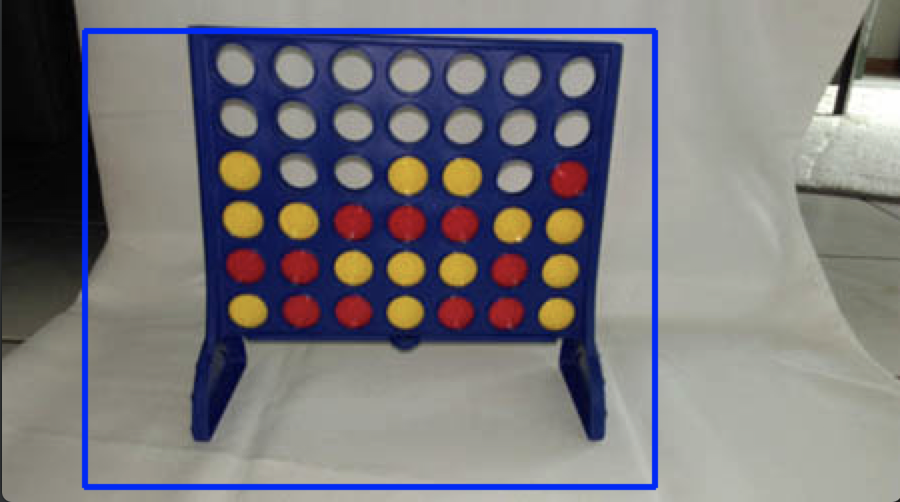
\includegraphics[width = .3\textwidth]{figures/detection.png}
  \caption{Baby in a Magnetoencephalograph. \parencite{babyMEG}}
  \label{fig:meg}
\end{figure}


 by color and pattern comparision.
The image is then cropped and undergoes various image processing steps, such as wrapping, contrast enhancement and color channel extraction.
The current board configuration can then be read and converted to a computer readable format by thresholded color comparision.

\subsection{State representation}
Theoretically, we need at least $\lfloor \log_2 3^{6\cdot 7} \rfloor = 67$ bit to store the entire game state, so we could just use a single
128-bit integer to store it.
However, we chose a slightly longer representation by storing the state $s$ in an array of $7$ 16-bit integers $s_i$, one for each column (14 bytes or 112 bit in total).
In each of these integers $s_i$ we assigned two bits for each row of the board, beginning at the lowest two bits with the lowest row.
For every cell, we set the assigned bits to $01$ to represent a coin of player 1, $10$ to represent a coin of player 2 and $00$ to represent an empty cell.

We can now for example efficiently check if a column is full by just checking if the bits of the highest row are set or if the integer value of the column exceeds $0b01000000000$.
Modifying the board and checking for winning positions now just requires some simple bit-wise operations on these integers.

\subsection{Learning}
Our approach to learning the game follows standard reinforcement learning methods.
Our training algorithm performs $N_i$ iterations and simulate $N_g$ games in every iteration.
In each of the simulated games, the moves are determined by a neural network that we will describe in detail below.
The current board state is taken as the input to the neural network and one of the allowed next moves is determined randomly using, weighted by the results of the neural network.
We have only added one single bit of game knowledge to this algorithm: If one of the allowed next moves is a winning move, that move will always be performed.
After the move has ended, a total reward of the end position will be calculated.
We used a reward of $100$ for winning, $-100$ for losing and $-10$ for a draw.

This reward will then be used by the employed algorithms for automatic differentiation and optimization\cite{Adam}, implemented by the software library PyTorch\cite{PyTorch}.

The neural network is constructed of a layer of 42 input neurons, one for each cell of the board, then two layers of 64 neurons each and finally a layer of 8 output neurons, one for each column of the board that the next move could put a coin into.

During the simulations, we experimented with different types of training opponents: random play, random play with winning move recognition and self-play.
In the first case, the opponent just randomly chooses one of the possible moves while in the second case, a random move is chosen except in situations where there is a move that leads to a win of the opponent.
In the third case, the same algorithm and neural network that we train and use for the first player is used for playing both sides (but only the actions of the first player are used for learning).
To avoid the self-play method to just play the same game over and over again, we add some random noise to the decisions of the opponent.

It can be shown that with perfect play on both sides, the first player to insert a coin will always win if and only if they insert their coin in one of the columns adjacent to the middle.
If the first coin is inserted in the outer columns of the game, the second player can win with perfect play.

The consequence of this is that if our learning agent learns the perfect strategy, we would still only see a winning rate of $50\%$ if we randomly
let the agent and its opponent begin.
For simplicity and more understandable results, we therefore assume that our agent always begins the game.

%-------------------------------------------------------------------------
\section{Results}

\subsection{Vision}
Processing time is $< 0.3$ s (i7-4790K CPU @ 4.00GHz) per image.

\subsection{Learning}
Our training algorithm was mainly CPU-bound and using a GPU for tensor
operation did not pose a speed-up since the time wasn't lost in the neural
network computation but in the game logic (e.g. checks for winning position).
We tried to quickly port our Python game logic code to Cython code but were
unable to achieve a speed-up without investing more engineering effort.
In the end, we were able to simulate $N_g = 250$ games and learn from
them within $4\mathrm{s}$ on a fast desktop CPU (i7-4790K @ 4.00 GHz)
or within $8 \mathrm{s}$ on a regular notebook CPU (i5-3210M CPU @ 2.50GHz).

\begin{figure}[t]
    \begin{center}
		\noindent
		\makebox[3.25in]{
	   		%% Creator: Matplotlib, PGF backend
%%
%% To include the figure in your LaTeX document, write
%%   \input{<filename>.pgf}
%%
%% Make sure the required packages are loaded in your preamble
%%   \usepackage{pgf}
%%
%% Figures using additional raster images can only be included by \input if
%% they are in the same directory as the main LaTeX file. For loading figures
%% from other directories you can use the `import` package
%%   \usepackage{import}
%% and then include the figures with
%%   \import{<path to file>}{<filename>.pgf}
%%
%% Matplotlib used the following preamble
%%   \usepackage{fontspec}
%%   \setmainfont{DejaVu Serif}
%%   \setsansfont{DejaVu Sans}
%%   \setmonofont{DejaVu Sans Mono}
%%
\begingroup%
\makeatletter%
\begin{pgfpicture}%
\pgfpathrectangle{\pgfpointorigin}{\pgfqpoint{3.250000in}{3.000000in}}%
\pgfusepath{use as bounding box, clip}%
\begin{pgfscope}%
\pgfsetbuttcap%
\pgfsetmiterjoin%
\definecolor{currentfill}{rgb}{1.000000,1.000000,1.000000}%
\pgfsetfillcolor{currentfill}%
\pgfsetlinewidth{0.000000pt}%
\definecolor{currentstroke}{rgb}{1.000000,1.000000,1.000000}%
\pgfsetstrokecolor{currentstroke}%
\pgfsetdash{}{0pt}%
\pgfpathmoveto{\pgfqpoint{0.000000in}{0.000000in}}%
\pgfpathlineto{\pgfqpoint{3.250000in}{0.000000in}}%
\pgfpathlineto{\pgfqpoint{3.250000in}{3.000000in}}%
\pgfpathlineto{\pgfqpoint{0.000000in}{3.000000in}}%
\pgfpathclose%
\pgfusepath{fill}%
\end{pgfscope}%
\begin{pgfscope}%
\pgfsetbuttcap%
\pgfsetmiterjoin%
\definecolor{currentfill}{rgb}{1.000000,1.000000,1.000000}%
\pgfsetfillcolor{currentfill}%
\pgfsetlinewidth{0.000000pt}%
\definecolor{currentstroke}{rgb}{0.000000,0.000000,0.000000}%
\pgfsetstrokecolor{currentstroke}%
\pgfsetstrokeopacity{0.000000}%
\pgfsetdash{}{0pt}%
\pgfpathmoveto{\pgfqpoint{0.706528in}{0.582778in}}%
\pgfpathlineto{\pgfqpoint{3.065000in}{0.582778in}}%
\pgfpathlineto{\pgfqpoint{3.065000in}{2.795000in}}%
\pgfpathlineto{\pgfqpoint{0.706528in}{2.795000in}}%
\pgfpathclose%
\pgfusepath{fill}%
\end{pgfscope}%
\begin{pgfscope}%
\pgfsetbuttcap%
\pgfsetroundjoin%
\definecolor{currentfill}{rgb}{0.000000,0.000000,0.000000}%
\pgfsetfillcolor{currentfill}%
\pgfsetlinewidth{0.803000pt}%
\definecolor{currentstroke}{rgb}{0.000000,0.000000,0.000000}%
\pgfsetstrokecolor{currentstroke}%
\pgfsetdash{}{0pt}%
\pgfsys@defobject{currentmarker}{\pgfqpoint{0.000000in}{-0.048611in}}{\pgfqpoint{0.000000in}{0.000000in}}{%
\pgfpathmoveto{\pgfqpoint{0.000000in}{0.000000in}}%
\pgfpathlineto{\pgfqpoint{0.000000in}{-0.048611in}}%
\pgfusepath{stroke,fill}%
}%
\begin{pgfscope}%
\pgfsys@transformshift{0.813731in}{0.582778in}%
\pgfsys@useobject{currentmarker}{}%
\end{pgfscope}%
\end{pgfscope}%
\begin{pgfscope}%
\pgftext[x=0.813731in,y=0.485556in,,top]{\sffamily\fontsize{10.000000}{12.000000}\selectfont 0}%
\end{pgfscope}%
\begin{pgfscope}%
\pgfsetbuttcap%
\pgfsetroundjoin%
\definecolor{currentfill}{rgb}{0.000000,0.000000,0.000000}%
\pgfsetfillcolor{currentfill}%
\pgfsetlinewidth{0.803000pt}%
\definecolor{currentstroke}{rgb}{0.000000,0.000000,0.000000}%
\pgfsetstrokecolor{currentstroke}%
\pgfsetdash{}{0pt}%
\pgfsys@defobject{currentmarker}{\pgfqpoint{0.000000in}{-0.048611in}}{\pgfqpoint{0.000000in}{0.000000in}}{%
\pgfpathmoveto{\pgfqpoint{0.000000in}{0.000000in}}%
\pgfpathlineto{\pgfqpoint{0.000000in}{-0.048611in}}%
\pgfusepath{stroke,fill}%
}%
\begin{pgfscope}%
\pgfsys@transformshift{1.344440in}{0.582778in}%
\pgfsys@useobject{currentmarker}{}%
\end{pgfscope}%
\end{pgfscope}%
\begin{pgfscope}%
\pgftext[x=1.344440in,y=0.485556in,,top]{\sffamily\fontsize{10.000000}{12.000000}\selectfont 25}%
\end{pgfscope}%
\begin{pgfscope}%
\pgfsetbuttcap%
\pgfsetroundjoin%
\definecolor{currentfill}{rgb}{0.000000,0.000000,0.000000}%
\pgfsetfillcolor{currentfill}%
\pgfsetlinewidth{0.803000pt}%
\definecolor{currentstroke}{rgb}{0.000000,0.000000,0.000000}%
\pgfsetstrokecolor{currentstroke}%
\pgfsetdash{}{0pt}%
\pgfsys@defobject{currentmarker}{\pgfqpoint{0.000000in}{-0.048611in}}{\pgfqpoint{0.000000in}{0.000000in}}{%
\pgfpathmoveto{\pgfqpoint{0.000000in}{0.000000in}}%
\pgfpathlineto{\pgfqpoint{0.000000in}{-0.048611in}}%
\pgfusepath{stroke,fill}%
}%
\begin{pgfscope}%
\pgfsys@transformshift{1.875150in}{0.582778in}%
\pgfsys@useobject{currentmarker}{}%
\end{pgfscope}%
\end{pgfscope}%
\begin{pgfscope}%
\pgftext[x=1.875150in,y=0.485556in,,top]{\sffamily\fontsize{10.000000}{12.000000}\selectfont 50}%
\end{pgfscope}%
\begin{pgfscope}%
\pgfsetbuttcap%
\pgfsetroundjoin%
\definecolor{currentfill}{rgb}{0.000000,0.000000,0.000000}%
\pgfsetfillcolor{currentfill}%
\pgfsetlinewidth{0.803000pt}%
\definecolor{currentstroke}{rgb}{0.000000,0.000000,0.000000}%
\pgfsetstrokecolor{currentstroke}%
\pgfsetdash{}{0pt}%
\pgfsys@defobject{currentmarker}{\pgfqpoint{0.000000in}{-0.048611in}}{\pgfqpoint{0.000000in}{0.000000in}}{%
\pgfpathmoveto{\pgfqpoint{0.000000in}{0.000000in}}%
\pgfpathlineto{\pgfqpoint{0.000000in}{-0.048611in}}%
\pgfusepath{stroke,fill}%
}%
\begin{pgfscope}%
\pgfsys@transformshift{2.405859in}{0.582778in}%
\pgfsys@useobject{currentmarker}{}%
\end{pgfscope}%
\end{pgfscope}%
\begin{pgfscope}%
\pgftext[x=2.405859in,y=0.485556in,,top]{\sffamily\fontsize{10.000000}{12.000000}\selectfont 75}%
\end{pgfscope}%
\begin{pgfscope}%
\pgfsetbuttcap%
\pgfsetroundjoin%
\definecolor{currentfill}{rgb}{0.000000,0.000000,0.000000}%
\pgfsetfillcolor{currentfill}%
\pgfsetlinewidth{0.803000pt}%
\definecolor{currentstroke}{rgb}{0.000000,0.000000,0.000000}%
\pgfsetstrokecolor{currentstroke}%
\pgfsetdash{}{0pt}%
\pgfsys@defobject{currentmarker}{\pgfqpoint{0.000000in}{-0.048611in}}{\pgfqpoint{0.000000in}{0.000000in}}{%
\pgfpathmoveto{\pgfqpoint{0.000000in}{0.000000in}}%
\pgfpathlineto{\pgfqpoint{0.000000in}{-0.048611in}}%
\pgfusepath{stroke,fill}%
}%
\begin{pgfscope}%
\pgfsys@transformshift{2.936568in}{0.582778in}%
\pgfsys@useobject{currentmarker}{}%
\end{pgfscope}%
\end{pgfscope}%
\begin{pgfscope}%
\pgftext[x=2.936568in,y=0.485556in,,top]{\sffamily\fontsize{10.000000}{12.000000}\selectfont 100}%
\end{pgfscope}%
\begin{pgfscope}%
\pgftext[x=1.885764in,y=0.295587in,,top]{\sffamily\fontsize{10.000000}{12.000000}\selectfont Iteration}%
\end{pgfscope}%
\begin{pgfscope}%
\pgfsetbuttcap%
\pgfsetroundjoin%
\definecolor{currentfill}{rgb}{0.000000,0.000000,0.000000}%
\pgfsetfillcolor{currentfill}%
\pgfsetlinewidth{0.803000pt}%
\definecolor{currentstroke}{rgb}{0.000000,0.000000,0.000000}%
\pgfsetstrokecolor{currentstroke}%
\pgfsetdash{}{0pt}%
\pgfsys@defobject{currentmarker}{\pgfqpoint{-0.048611in}{0.000000in}}{\pgfqpoint{0.000000in}{0.000000in}}{%
\pgfpathmoveto{\pgfqpoint{0.000000in}{0.000000in}}%
\pgfpathlineto{\pgfqpoint{-0.048611in}{0.000000in}}%
\pgfusepath{stroke,fill}%
}%
\begin{pgfscope}%
\pgfsys@transformshift{0.706528in}{0.582778in}%
\pgfsys@useobject{currentmarker}{}%
\end{pgfscope}%
\end{pgfscope}%
\begin{pgfscope}%
\pgftext[x=0.520940in,y=0.530016in,left,base]{\sffamily\fontsize{10.000000}{12.000000}\selectfont 0}%
\end{pgfscope}%
\begin{pgfscope}%
\pgfsetbuttcap%
\pgfsetroundjoin%
\definecolor{currentfill}{rgb}{0.000000,0.000000,0.000000}%
\pgfsetfillcolor{currentfill}%
\pgfsetlinewidth{0.803000pt}%
\definecolor{currentstroke}{rgb}{0.000000,0.000000,0.000000}%
\pgfsetstrokecolor{currentstroke}%
\pgfsetdash{}{0pt}%
\pgfsys@defobject{currentmarker}{\pgfqpoint{-0.048611in}{0.000000in}}{\pgfqpoint{0.000000in}{0.000000in}}{%
\pgfpathmoveto{\pgfqpoint{0.000000in}{0.000000in}}%
\pgfpathlineto{\pgfqpoint{-0.048611in}{0.000000in}}%
\pgfusepath{stroke,fill}%
}%
\begin{pgfscope}%
\pgfsys@transformshift{0.706528in}{1.025222in}%
\pgfsys@useobject{currentmarker}{}%
\end{pgfscope}%
\end{pgfscope}%
\begin{pgfscope}%
\pgftext[x=0.432575in,y=0.972461in,left,base]{\sffamily\fontsize{10.000000}{12.000000}\selectfont 20}%
\end{pgfscope}%
\begin{pgfscope}%
\pgfsetbuttcap%
\pgfsetroundjoin%
\definecolor{currentfill}{rgb}{0.000000,0.000000,0.000000}%
\pgfsetfillcolor{currentfill}%
\pgfsetlinewidth{0.803000pt}%
\definecolor{currentstroke}{rgb}{0.000000,0.000000,0.000000}%
\pgfsetstrokecolor{currentstroke}%
\pgfsetdash{}{0pt}%
\pgfsys@defobject{currentmarker}{\pgfqpoint{-0.048611in}{0.000000in}}{\pgfqpoint{0.000000in}{0.000000in}}{%
\pgfpathmoveto{\pgfqpoint{0.000000in}{0.000000in}}%
\pgfpathlineto{\pgfqpoint{-0.048611in}{0.000000in}}%
\pgfusepath{stroke,fill}%
}%
\begin{pgfscope}%
\pgfsys@transformshift{0.706528in}{1.467667in}%
\pgfsys@useobject{currentmarker}{}%
\end{pgfscope}%
\end{pgfscope}%
\begin{pgfscope}%
\pgftext[x=0.432575in,y=1.414905in,left,base]{\sffamily\fontsize{10.000000}{12.000000}\selectfont 40}%
\end{pgfscope}%
\begin{pgfscope}%
\pgfsetbuttcap%
\pgfsetroundjoin%
\definecolor{currentfill}{rgb}{0.000000,0.000000,0.000000}%
\pgfsetfillcolor{currentfill}%
\pgfsetlinewidth{0.803000pt}%
\definecolor{currentstroke}{rgb}{0.000000,0.000000,0.000000}%
\pgfsetstrokecolor{currentstroke}%
\pgfsetdash{}{0pt}%
\pgfsys@defobject{currentmarker}{\pgfqpoint{-0.048611in}{0.000000in}}{\pgfqpoint{0.000000in}{0.000000in}}{%
\pgfpathmoveto{\pgfqpoint{0.000000in}{0.000000in}}%
\pgfpathlineto{\pgfqpoint{-0.048611in}{0.000000in}}%
\pgfusepath{stroke,fill}%
}%
\begin{pgfscope}%
\pgfsys@transformshift{0.706528in}{1.910111in}%
\pgfsys@useobject{currentmarker}{}%
\end{pgfscope}%
\end{pgfscope}%
\begin{pgfscope}%
\pgftext[x=0.432575in,y=1.857350in,left,base]{\sffamily\fontsize{10.000000}{12.000000}\selectfont 60}%
\end{pgfscope}%
\begin{pgfscope}%
\pgfsetbuttcap%
\pgfsetroundjoin%
\definecolor{currentfill}{rgb}{0.000000,0.000000,0.000000}%
\pgfsetfillcolor{currentfill}%
\pgfsetlinewidth{0.803000pt}%
\definecolor{currentstroke}{rgb}{0.000000,0.000000,0.000000}%
\pgfsetstrokecolor{currentstroke}%
\pgfsetdash{}{0pt}%
\pgfsys@defobject{currentmarker}{\pgfqpoint{-0.048611in}{0.000000in}}{\pgfqpoint{0.000000in}{0.000000in}}{%
\pgfpathmoveto{\pgfqpoint{0.000000in}{0.000000in}}%
\pgfpathlineto{\pgfqpoint{-0.048611in}{0.000000in}}%
\pgfusepath{stroke,fill}%
}%
\begin{pgfscope}%
\pgfsys@transformshift{0.706528in}{2.352556in}%
\pgfsys@useobject{currentmarker}{}%
\end{pgfscope}%
\end{pgfscope}%
\begin{pgfscope}%
\pgftext[x=0.432575in,y=2.299794in,left,base]{\sffamily\fontsize{10.000000}{12.000000}\selectfont 80}%
\end{pgfscope}%
\begin{pgfscope}%
\pgfsetbuttcap%
\pgfsetroundjoin%
\definecolor{currentfill}{rgb}{0.000000,0.000000,0.000000}%
\pgfsetfillcolor{currentfill}%
\pgfsetlinewidth{0.803000pt}%
\definecolor{currentstroke}{rgb}{0.000000,0.000000,0.000000}%
\pgfsetstrokecolor{currentstroke}%
\pgfsetdash{}{0pt}%
\pgfsys@defobject{currentmarker}{\pgfqpoint{-0.048611in}{0.000000in}}{\pgfqpoint{0.000000in}{0.000000in}}{%
\pgfpathmoveto{\pgfqpoint{0.000000in}{0.000000in}}%
\pgfpathlineto{\pgfqpoint{-0.048611in}{0.000000in}}%
\pgfusepath{stroke,fill}%
}%
\begin{pgfscope}%
\pgfsys@transformshift{0.706528in}{2.795000in}%
\pgfsys@useobject{currentmarker}{}%
\end{pgfscope}%
\end{pgfscope}%
\begin{pgfscope}%
\pgftext[x=0.344210in,y=2.742238in,left,base]{\sffamily\fontsize{10.000000}{12.000000}\selectfont 100}%
\end{pgfscope}%
\begin{pgfscope}%
\pgftext[x=0.288654in,y=1.688889in,,bottom,rotate=90.000000]{\sffamily\fontsize{10.000000}{12.000000}\selectfont Winning rate (\%)}%
\end{pgfscope}%
\begin{pgfscope}%
\pgfpathrectangle{\pgfqpoint{0.706528in}{0.582778in}}{\pgfqpoint{2.358472in}{2.212222in}} %
\pgfusepath{clip}%
\pgfsetrectcap%
\pgfsetroundjoin%
\pgfsetlinewidth{1.505625pt}%
\definecolor{currentstroke}{rgb}{0.121569,0.466667,0.705882}%
\pgfsetstrokecolor{currentstroke}%
\pgfsetdash{}{0pt}%
\pgfpathmoveto{\pgfqpoint{0.813731in}{1.910111in}}%
\pgfpathlineto{\pgfqpoint{0.834959in}{2.060542in}}%
\pgfpathlineto{\pgfqpoint{0.856188in}{2.051693in}}%
\pgfpathlineto{\pgfqpoint{0.877416in}{1.989751in}}%
\pgfpathlineto{\pgfqpoint{0.898645in}{2.087089in}}%
\pgfpathlineto{\pgfqpoint{0.919873in}{2.122484in}}%
\pgfpathlineto{\pgfqpoint{0.941101in}{2.069391in}}%
\pgfpathlineto{\pgfqpoint{0.962330in}{1.980902in}}%
\pgfpathlineto{\pgfqpoint{0.983558in}{2.051693in}}%
\pgfpathlineto{\pgfqpoint{1.004786in}{1.945507in}}%
\pgfpathlineto{\pgfqpoint{1.026015in}{2.033996in}}%
\pgfpathlineto{\pgfqpoint{1.047243in}{2.051693in}}%
\pgfpathlineto{\pgfqpoint{1.068472in}{2.042844in}}%
\pgfpathlineto{\pgfqpoint{1.089700in}{1.901262in}}%
\pgfpathlineto{\pgfqpoint{1.110928in}{1.662342in}}%
\pgfpathlineto{\pgfqpoint{1.132157in}{1.839320in}}%
\pgfpathlineto{\pgfqpoint{1.153385in}{2.033996in}}%
\pgfpathlineto{\pgfqpoint{1.174613in}{1.565004in}}%
\pgfpathlineto{\pgfqpoint{1.195842in}{1.388027in}}%
\pgfpathlineto{\pgfqpoint{1.217070in}{1.467667in}}%
\pgfpathlineto{\pgfqpoint{1.238299in}{2.122484in}}%
\pgfpathlineto{\pgfqpoint{1.259527in}{1.963204in}}%
\pgfpathlineto{\pgfqpoint{1.280755in}{1.874716in}}%
\pgfpathlineto{\pgfqpoint{1.301984in}{2.069391in}}%
\pgfpathlineto{\pgfqpoint{1.323212in}{2.016298in}}%
\pgfpathlineto{\pgfqpoint{1.344440in}{1.963204in}}%
\pgfpathlineto{\pgfqpoint{1.365669in}{1.927809in}}%
\pgfpathlineto{\pgfqpoint{1.386897in}{1.989751in}}%
\pgfpathlineto{\pgfqpoint{1.408126in}{1.927809in}}%
\pgfpathlineto{\pgfqpoint{1.429354in}{1.901262in}}%
\pgfpathlineto{\pgfqpoint{1.450582in}{1.343782in}}%
\pgfpathlineto{\pgfqpoint{1.471811in}{1.458818in}}%
\pgfpathlineto{\pgfqpoint{1.493039in}{1.963204in}}%
\pgfpathlineto{\pgfqpoint{1.514267in}{1.963204in}}%
\pgfpathlineto{\pgfqpoint{1.535496in}{2.087089in}}%
\pgfpathlineto{\pgfqpoint{1.556724in}{1.883564in}}%
\pgfpathlineto{\pgfqpoint{1.577952in}{1.989751in}}%
\pgfpathlineto{\pgfqpoint{1.599181in}{1.963204in}}%
\pgfpathlineto{\pgfqpoint{1.620409in}{2.042844in}}%
\pgfpathlineto{\pgfqpoint{1.641638in}{1.901262in}}%
\pgfpathlineto{\pgfqpoint{1.662866in}{1.954356in}}%
\pgfpathlineto{\pgfqpoint{1.684094in}{2.025147in}}%
\pgfpathlineto{\pgfqpoint{1.705323in}{1.989751in}}%
\pgfpathlineto{\pgfqpoint{1.726551in}{2.025147in}}%
\pgfpathlineto{\pgfqpoint{1.747779in}{1.963204in}}%
\pgfpathlineto{\pgfqpoint{1.769008in}{2.025147in}}%
\pgfpathlineto{\pgfqpoint{1.790236in}{2.007449in}}%
\pgfpathlineto{\pgfqpoint{1.811465in}{2.007449in}}%
\pgfpathlineto{\pgfqpoint{1.832693in}{2.025147in}}%
\pgfpathlineto{\pgfqpoint{1.853921in}{1.963204in}}%
\pgfpathlineto{\pgfqpoint{1.875150in}{2.033996in}}%
\pgfpathlineto{\pgfqpoint{1.896378in}{2.122484in}}%
\pgfpathlineto{\pgfqpoint{1.917606in}{1.848169in}}%
\pgfpathlineto{\pgfqpoint{1.938835in}{1.927809in}}%
\pgfpathlineto{\pgfqpoint{1.960063in}{1.954356in}}%
\pgfpathlineto{\pgfqpoint{1.981292in}{1.927809in}}%
\pgfpathlineto{\pgfqpoint{2.002520in}{1.892413in}}%
\pgfpathlineto{\pgfqpoint{2.023748in}{1.927809in}}%
\pgfpathlineto{\pgfqpoint{2.044977in}{1.901262in}}%
\pgfpathlineto{\pgfqpoint{2.066205in}{2.016298in}}%
\pgfpathlineto{\pgfqpoint{2.087433in}{1.803924in}}%
\pgfpathlineto{\pgfqpoint{2.108662in}{2.042844in}}%
\pgfpathlineto{\pgfqpoint{2.129890in}{1.980902in}}%
\pgfpathlineto{\pgfqpoint{2.151119in}{1.945507in}}%
\pgfpathlineto{\pgfqpoint{2.172347in}{2.060542in}}%
\pgfpathlineto{\pgfqpoint{2.193575in}{2.007449in}}%
\pgfpathlineto{\pgfqpoint{2.214804in}{1.954356in}}%
\pgfpathlineto{\pgfqpoint{2.236032in}{1.963204in}}%
\pgfpathlineto{\pgfqpoint{2.257260in}{1.936658in}}%
\pgfpathlineto{\pgfqpoint{2.278489in}{1.892413in}}%
\pgfpathlineto{\pgfqpoint{2.299717in}{2.060542in}}%
\pgfpathlineto{\pgfqpoint{2.320946in}{1.972053in}}%
\pgfpathlineto{\pgfqpoint{2.342174in}{1.892413in}}%
\pgfpathlineto{\pgfqpoint{2.363402in}{2.033996in}}%
\pgfpathlineto{\pgfqpoint{2.384631in}{1.812773in}}%
\pgfpathlineto{\pgfqpoint{2.405859in}{1.980902in}}%
\pgfpathlineto{\pgfqpoint{2.427087in}{1.865867in}}%
\pgfpathlineto{\pgfqpoint{2.448316in}{2.007449in}}%
\pgfpathlineto{\pgfqpoint{2.469544in}{2.051693in}}%
\pgfpathlineto{\pgfqpoint{2.490773in}{1.963204in}}%
\pgfpathlineto{\pgfqpoint{2.512001in}{2.007449in}}%
\pgfpathlineto{\pgfqpoint{2.533229in}{1.759680in}}%
\pgfpathlineto{\pgfqpoint{2.554458in}{2.087089in}}%
\pgfpathlineto{\pgfqpoint{2.575686in}{1.857018in}}%
\pgfpathlineto{\pgfqpoint{2.596914in}{1.936658in}}%
\pgfpathlineto{\pgfqpoint{2.618143in}{1.927809in}}%
\pgfpathlineto{\pgfqpoint{2.639371in}{1.998600in}}%
\pgfpathlineto{\pgfqpoint{2.660599in}{2.033996in}}%
\pgfpathlineto{\pgfqpoint{2.681828in}{1.892413in}}%
\pgfpathlineto{\pgfqpoint{2.703056in}{1.963204in}}%
\pgfpathlineto{\pgfqpoint{2.724285in}{2.069391in}}%
\pgfpathlineto{\pgfqpoint{2.745513in}{1.927809in}}%
\pgfpathlineto{\pgfqpoint{2.766741in}{1.927809in}}%
\pgfpathlineto{\pgfqpoint{2.787970in}{1.989751in}}%
\pgfpathlineto{\pgfqpoint{2.809198in}{1.927809in}}%
\pgfpathlineto{\pgfqpoint{2.830426in}{1.963204in}}%
\pgfpathlineto{\pgfqpoint{2.851655in}{1.972053in}}%
\pgfpathlineto{\pgfqpoint{2.872883in}{1.812773in}}%
\pgfpathlineto{\pgfqpoint{2.894112in}{1.972053in}}%
\pgfpathlineto{\pgfqpoint{2.915340in}{1.989751in}}%
\pgfpathlineto{\pgfqpoint{2.936568in}{1.954356in}}%
\pgfpathlineto{\pgfqpoint{2.957797in}{1.857018in}}%
\pgfusepath{stroke}%
\end{pgfscope}%
\begin{pgfscope}%
\pgfsetrectcap%
\pgfsetmiterjoin%
\pgfsetlinewidth{0.803000pt}%
\definecolor{currentstroke}{rgb}{0.000000,0.000000,0.000000}%
\pgfsetstrokecolor{currentstroke}%
\pgfsetdash{}{0pt}%
\pgfpathmoveto{\pgfqpoint{0.706528in}{0.582778in}}%
\pgfpathlineto{\pgfqpoint{0.706528in}{2.795000in}}%
\pgfusepath{stroke}%
\end{pgfscope}%
\begin{pgfscope}%
\pgfsetrectcap%
\pgfsetmiterjoin%
\pgfsetlinewidth{0.803000pt}%
\definecolor{currentstroke}{rgb}{0.000000,0.000000,0.000000}%
\pgfsetstrokecolor{currentstroke}%
\pgfsetdash{}{0pt}%
\pgfpathmoveto{\pgfqpoint{3.065000in}{0.582778in}}%
\pgfpathlineto{\pgfqpoint{3.065000in}{2.795000in}}%
\pgfusepath{stroke}%
\end{pgfscope}%
\begin{pgfscope}%
\pgfsetrectcap%
\pgfsetmiterjoin%
\pgfsetlinewidth{0.803000pt}%
\definecolor{currentstroke}{rgb}{0.000000,0.000000,0.000000}%
\pgfsetstrokecolor{currentstroke}%
\pgfsetdash{}{0pt}%
\pgfpathmoveto{\pgfqpoint{0.706528in}{0.582778in}}%
\pgfpathlineto{\pgfqpoint{3.065000in}{0.582778in}}%
\pgfusepath{stroke}%
\end{pgfscope}%
\begin{pgfscope}%
\pgfsetrectcap%
\pgfsetmiterjoin%
\pgfsetlinewidth{0.803000pt}%
\definecolor{currentstroke}{rgb}{0.000000,0.000000,0.000000}%
\pgfsetstrokecolor{currentstroke}%
\pgfsetdash{}{0pt}%
\pgfpathmoveto{\pgfqpoint{0.706528in}{2.795000in}}%
\pgfpathlineto{\pgfqpoint{3.065000in}{2.795000in}}%
\pgfusepath{stroke}%
\end{pgfscope}%
\end{pgfpicture}%
\makeatother%
\endgroup%

		}
	\end{center}
    \caption{Play against random}
	\label{fig:long}
\end{figure}

TODO:
number of iterations, number of games
self-play vs random play
noise
reward strategies
%-------------------------------------------------------------------------
\section{Discussion}

{\small
\printbibliography
}

\end{document}
